\graphicspath{{capitulos/Capitulo2-Definicion-del-problema/recursos/}}

\section{Definición del problema} \label{apartado:2}

Tal y como se ha introducido antes, el proyecto ABACO pretende automatizar el proceso de creación de un horario de trabajo para
los distintos controladores del espacio aéreo de forma que, dada una sectorización de este, todos los sectores puedan ser
controlados siguiendo las pautas establecidas por el dominio del problema.

El control del espacio aéreo (también conocido como ATC, \textit{Air Trafic Control}) es una tarea que se lleva a cabo
en todos los aeropuertos con el fin de monitorizar los diferentes aviones que sobrevuelan una determinada zona del cielo,
de cara a garantizar la seguridad de sus rutas (lo que se denomina control de ruta), así como de sus aterrizajes
(que se llama control de aproximación o de área terminal), encargándose también de las comunicaciones de voz tanto
tierra-aire con los pilotos de las aeronaves (vía radio), como tierra-tierra con otros controladores u otro personal
de gestión (vía telefónica)~\cite{ENAIRE-web}.
La zona de trabajo de los controladores aéreos se denomina Centros de Control de Tráfico Aéreo, cuyos puestos de trabajo tienen
un aspecto similar al de la \autoref{fig:2:enaire-atc}.

\begin{figure}[htbp]
    \centering
    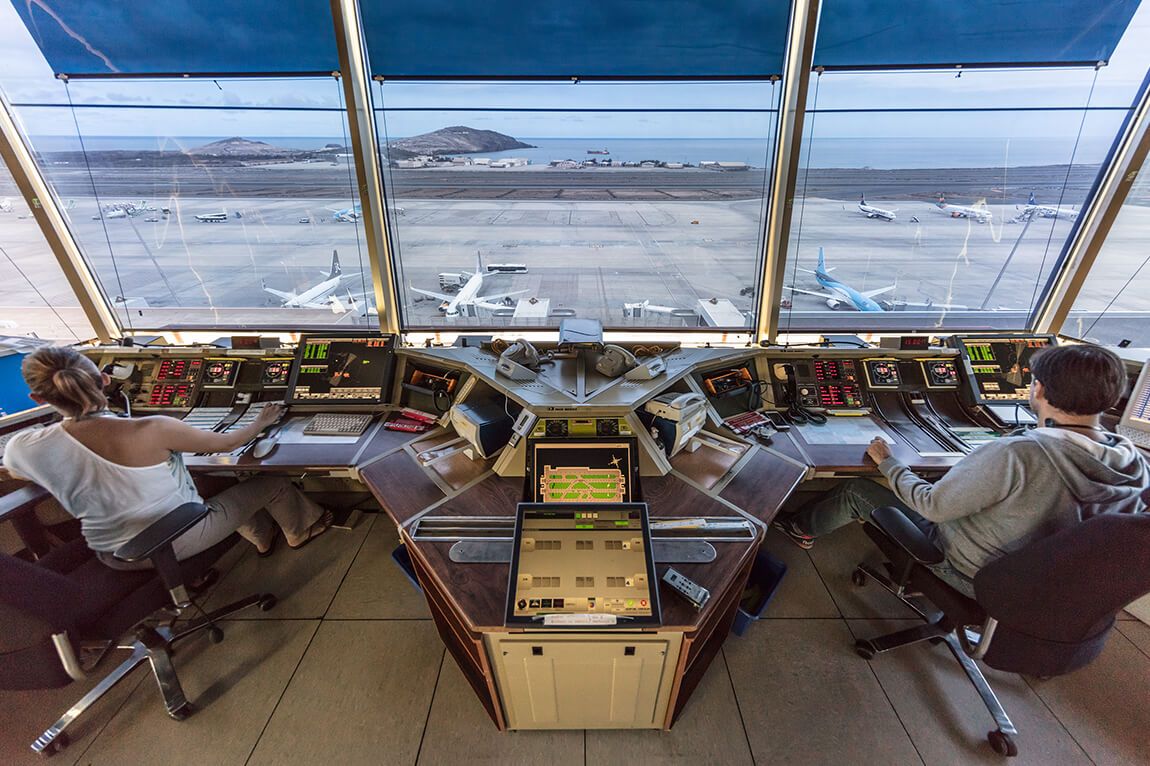
\includegraphics[width=0.7\linewidth]{ENAIRE-ATC}
    \caption{Fotografía de uno de los puestos de control, como puede verse está conformado por dos personas. Fuente: \url{https://muia.ml/wzfw8}}
    \label{fig:2:enaire-atc}
\end{figure}


\subsection{Sectores y sectorizaciones}
\label{section:2:sectores-y-sectorizacion}
Cada controlador tiene asignado durante un cierto intervalo de tiempo de su turno de trabajo, un sector que debe controlar.
Por ello, en primer lugar, explicaremos brevemente cómo se divide el espacio aéreo del territorio español, cuyo organismo
encargado de su gestión es precisamente ENAIRE
\footnote{\url{https://www.enaire.es/sobre_enaire/conoce_enaire/quienes_somos_ENAIRE}}.
Si bien la realidad es muy compleja, aquí únicamente describiremos una simplificación de la misma, omitiéndose
detalles técnicos de aviación que no son necesarios para la implementación del sistema.
\\

El espacio aéreo mundial se encuentra dividido en \textit{FIR}s (\textit{Flight Information Region}), áreas del
territorio sobre las que se mueven los diferentes aviones de cada compañía aérea de cada país, en la
\autoref{fig:2:fireuropa} puede verse gráficamente los límites de cada región. En el caso de España,
podemos ver que tiene control sobre 3 \textit{FIR}s: el de Barcelona, el de Madrid y el de Canarias, sin embargo,
a nivel nacional, existen algunas subdivisiones denominadas \textit{Dependencias} (ya que dependen del \textit{FIR}
en el que se encuentren), que permiten una mejor gestión del territorio. Las dependencias están constituidas por Centros de Control (\hyperref[ACC]{ACC}) (uno por cada Dependencia) y Torres de Control. Algunos de ellos aparecerán en los casos reales de prueba del sistema del \autoref{apartado:5}, así que los enumeramos a continuación:

\begin{figure}[htbp]
    \centering
    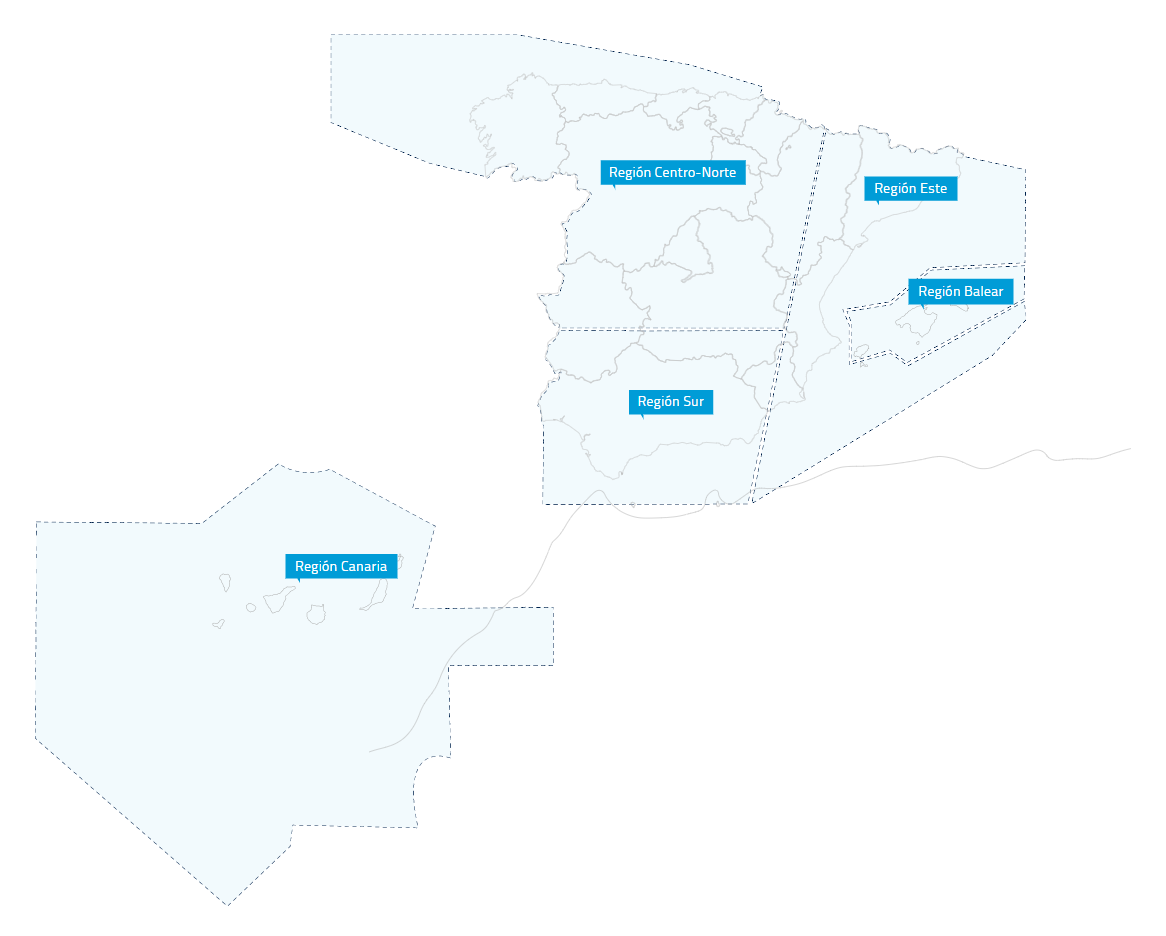
\includegraphics[width=0.7\linewidth]{Division-Espacio-Nacional}
    \caption{Simplificación de la división del espacio aéreo nacional}
    \label{fig:2:regiones}
\end{figure}

\begin{itemize}
    \item Barcelona
    \begin{itemize}
        \item Barcelona RutaE
        \item Barcelona RutaW
        \item Barcelona TMA\footnote{Ver definición en la \hyperref[TMA]{\autoref{sec:Definiciones}}} ESTE
        \item Barcelona TMA NORTE
        \item Barcelona TMA OESTE
    \end{itemize}
    \item Canarias
    \begin{itemize}
        \item Canarias ACC App
        \item Canarias ACC Ruta
    \end{itemize}
    \item Madrid
    \begin{itemize}
        \item Madrid Ruta 1
        \item Madrid Ruta 2
        \item Madrid TMA NORTE
        \item Madrid TMA SUR
    \end{itemize}
    \item Malaga App
    \item Palma TACC
    \item Sevilla TACC
    \item  Valencia TACC TMA
\end{itemize}


\begin{figure}[htbp]
    \centering
    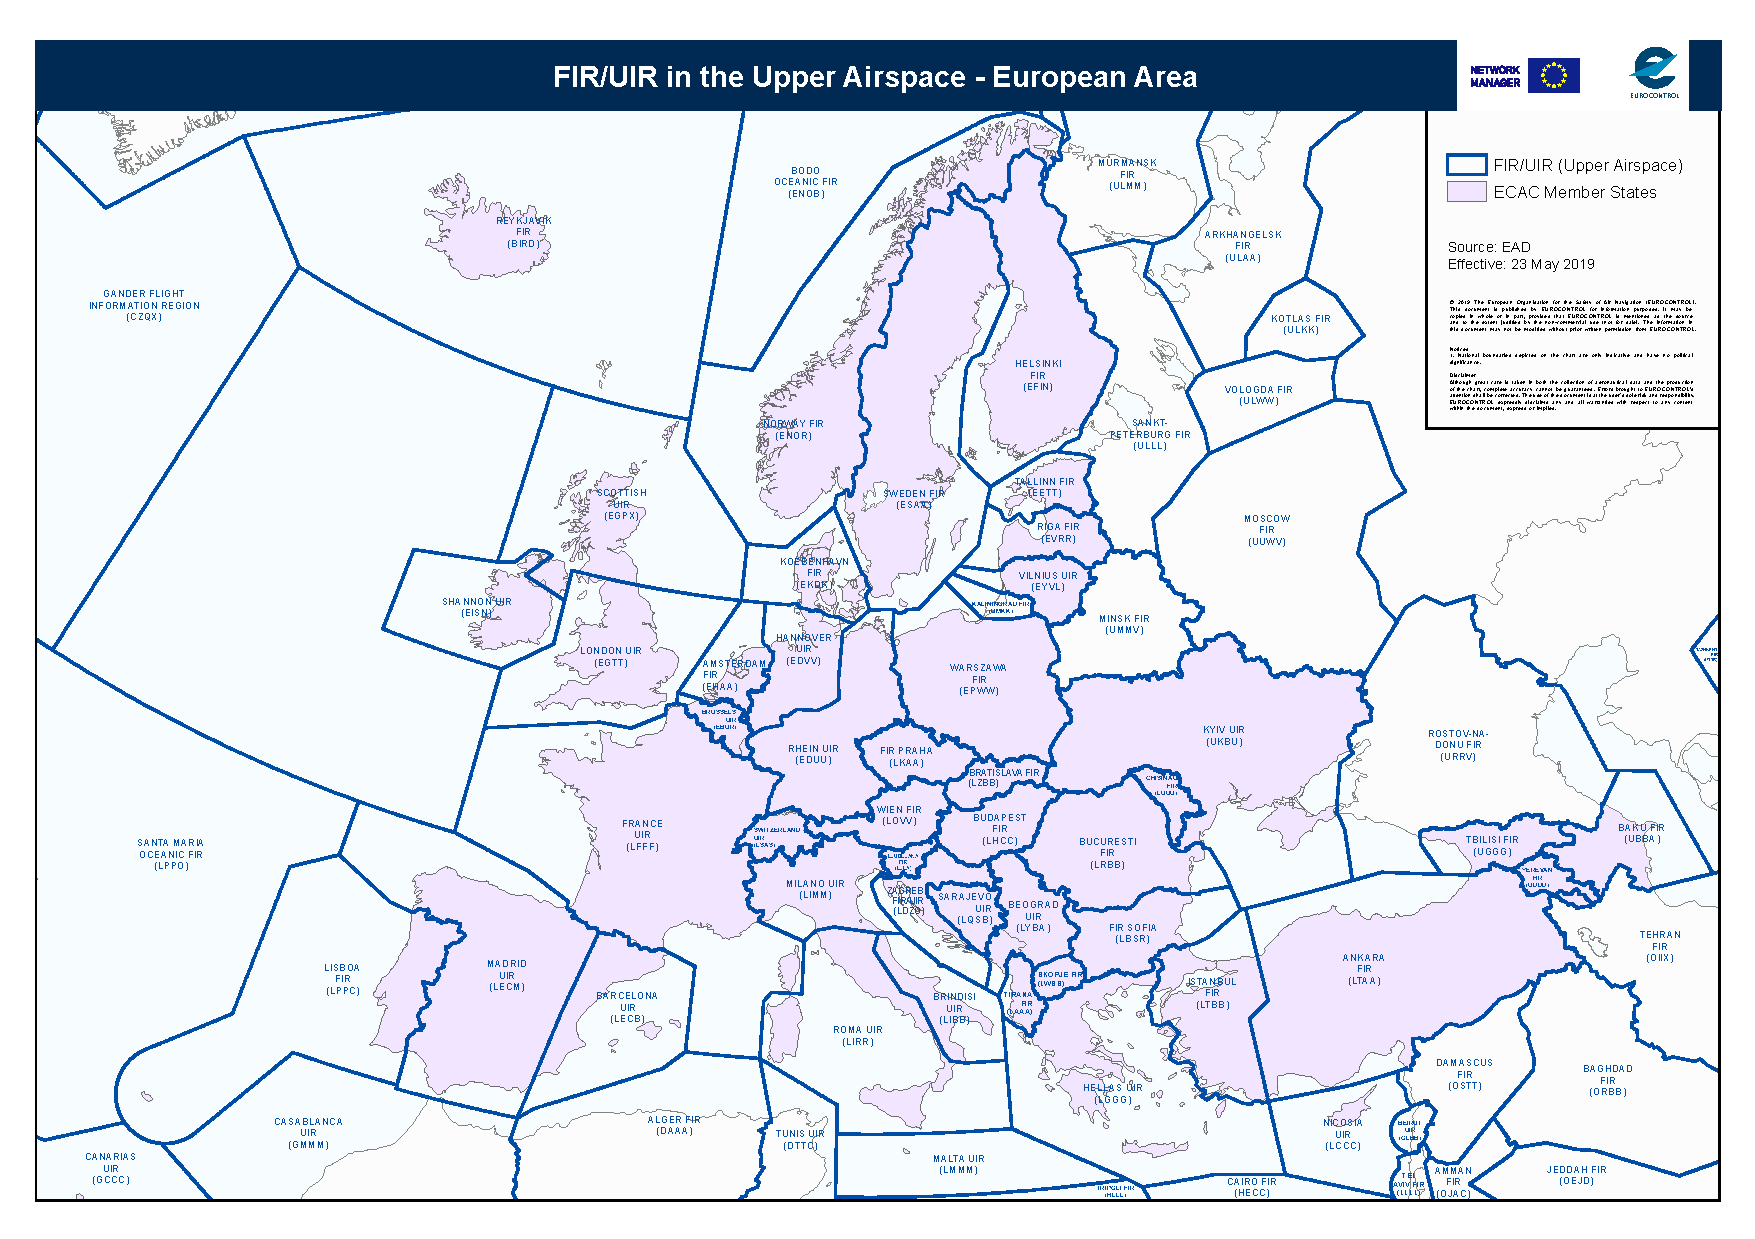
\includegraphics[width=\linewidth]{FIR_europa}
    \caption{FIRs de la zona europea. Fuente: EUROCONTROL}
    \label{fig:2:fireuropa}
\end{figure}

Cada una de estas Dependencias, está constituida por un cierto número de sectores, que se agrupan de forma que se cubra
todo el espacio de la zona, conformando lo que llamaremos una \textit{configuración o sectorización} concreta.
Existen varias configuraciones estandarizadas, de manera que dado un número de sectores, el espacio aéreo sea cubierto en su totalidad.
Por eso, las sectorizaciones se nombran utilizando dos caracteres: un número y una letra; el número indica precisamente
la cantidad de sectores de la configuración, mientras que la letra permite diferenciar entre dos posibles configuraciones
que emplean el mismo número de sectores.
\\

Por ejemplo, la configuración 3B de la dependencia MADRID Ruta 1 consta de los sectores LECMSAI, LECMBLI y LECMDPI,
mientras que una 3D consta de LECMSAN, LECMASI y LECMBDP. En ambos casos se utilizan tres sectores y el espacio cubierto
total es equivalente, como puede apreciarse en la \autoref{fig:2:comparativa3B-3D}.
De la misma forma, si utilizamos una configuración 5A, se utilizarían 5 sectores diferentes, pero el espacio aéreo a
controlar sería nuevamente equivalente, como se aprecia en la \autoref{fig:2:sectorizacion-5a}.
Nótese además, que los sectores LECMSAN (amarillo) y LECMASI (verde) son los mismo que los de la sectorización 3D (\autoref{fig:2:sectorizacion-3d})
pero el sector LECMBDP (azul) se ha dividido o \textit{abierto} en los sectores LECMBLI, LECMDGI y LECMPAI.
\\

\begin{figure}[htbp]
    \centering
    \begin{subfigure}{\linewidth}
        \centering
        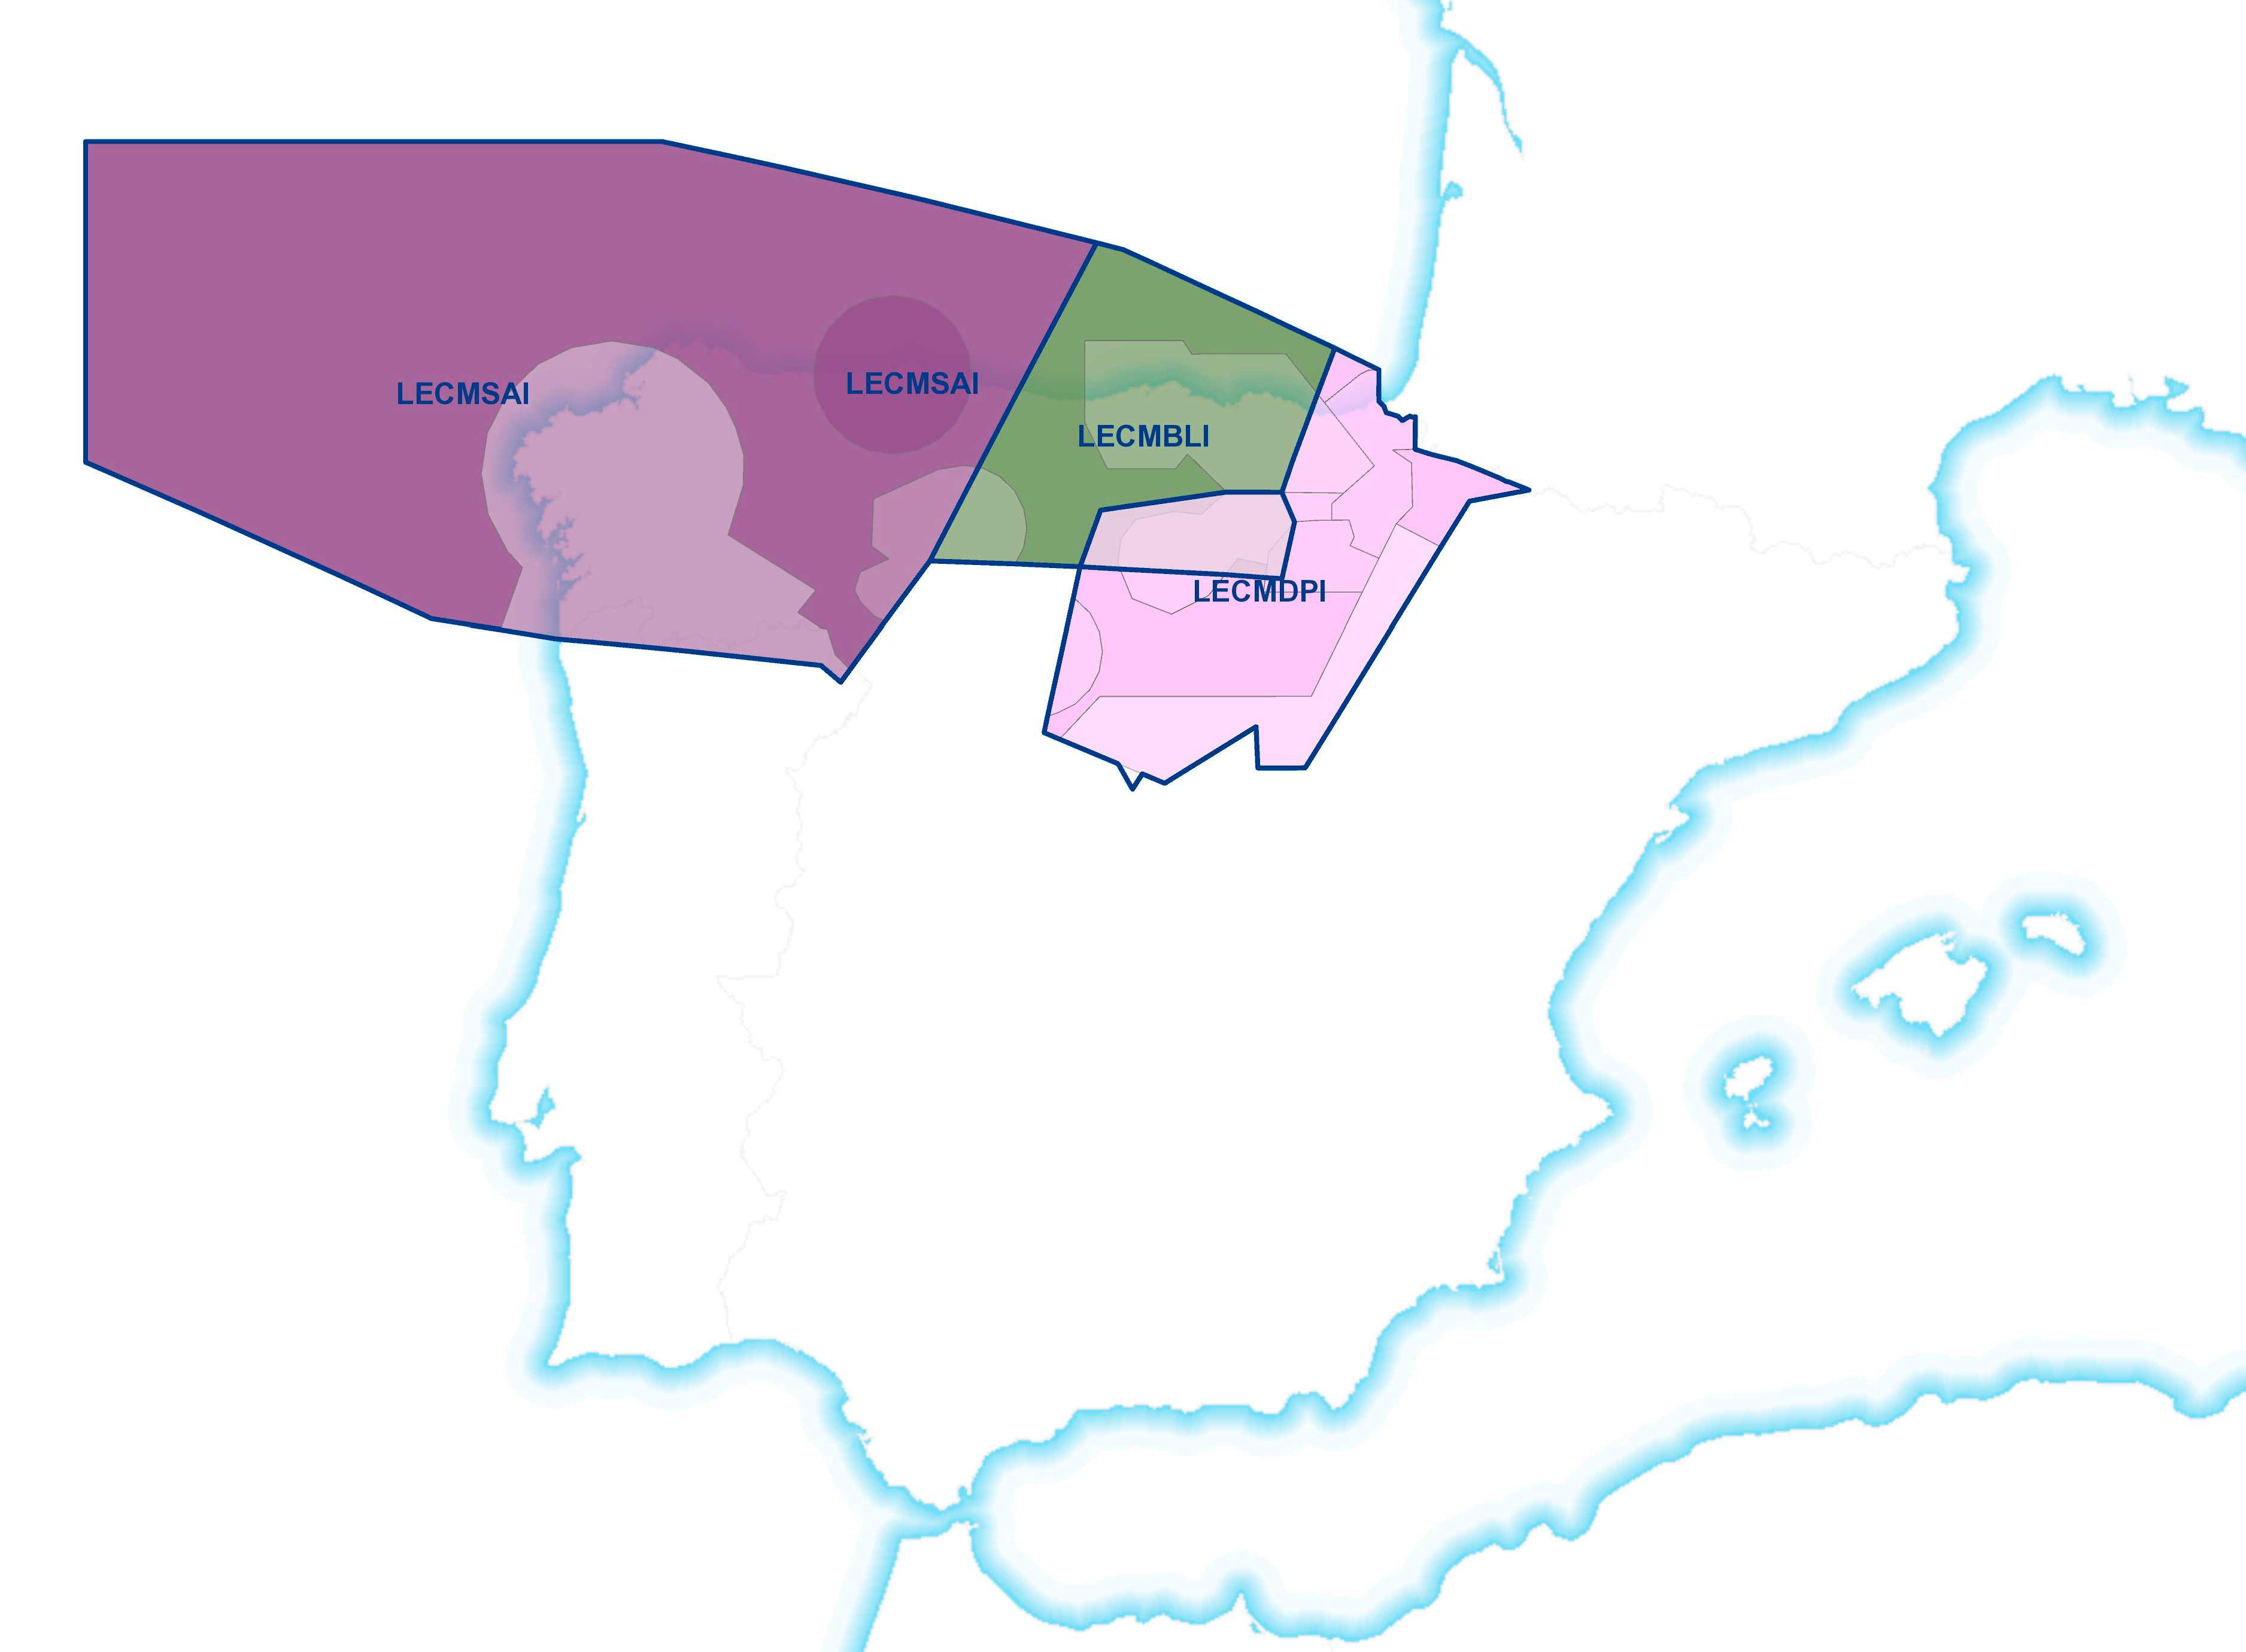
\includegraphics[width=0.6\linewidth]{sectorizacion-3B}
        \caption{sectorizacion 3B\linebreak}
        %	\label{fig:sectorizacion-3b}
    \end{subfigure}

    \begin{subfigure}{\linewidth}
        \centering
        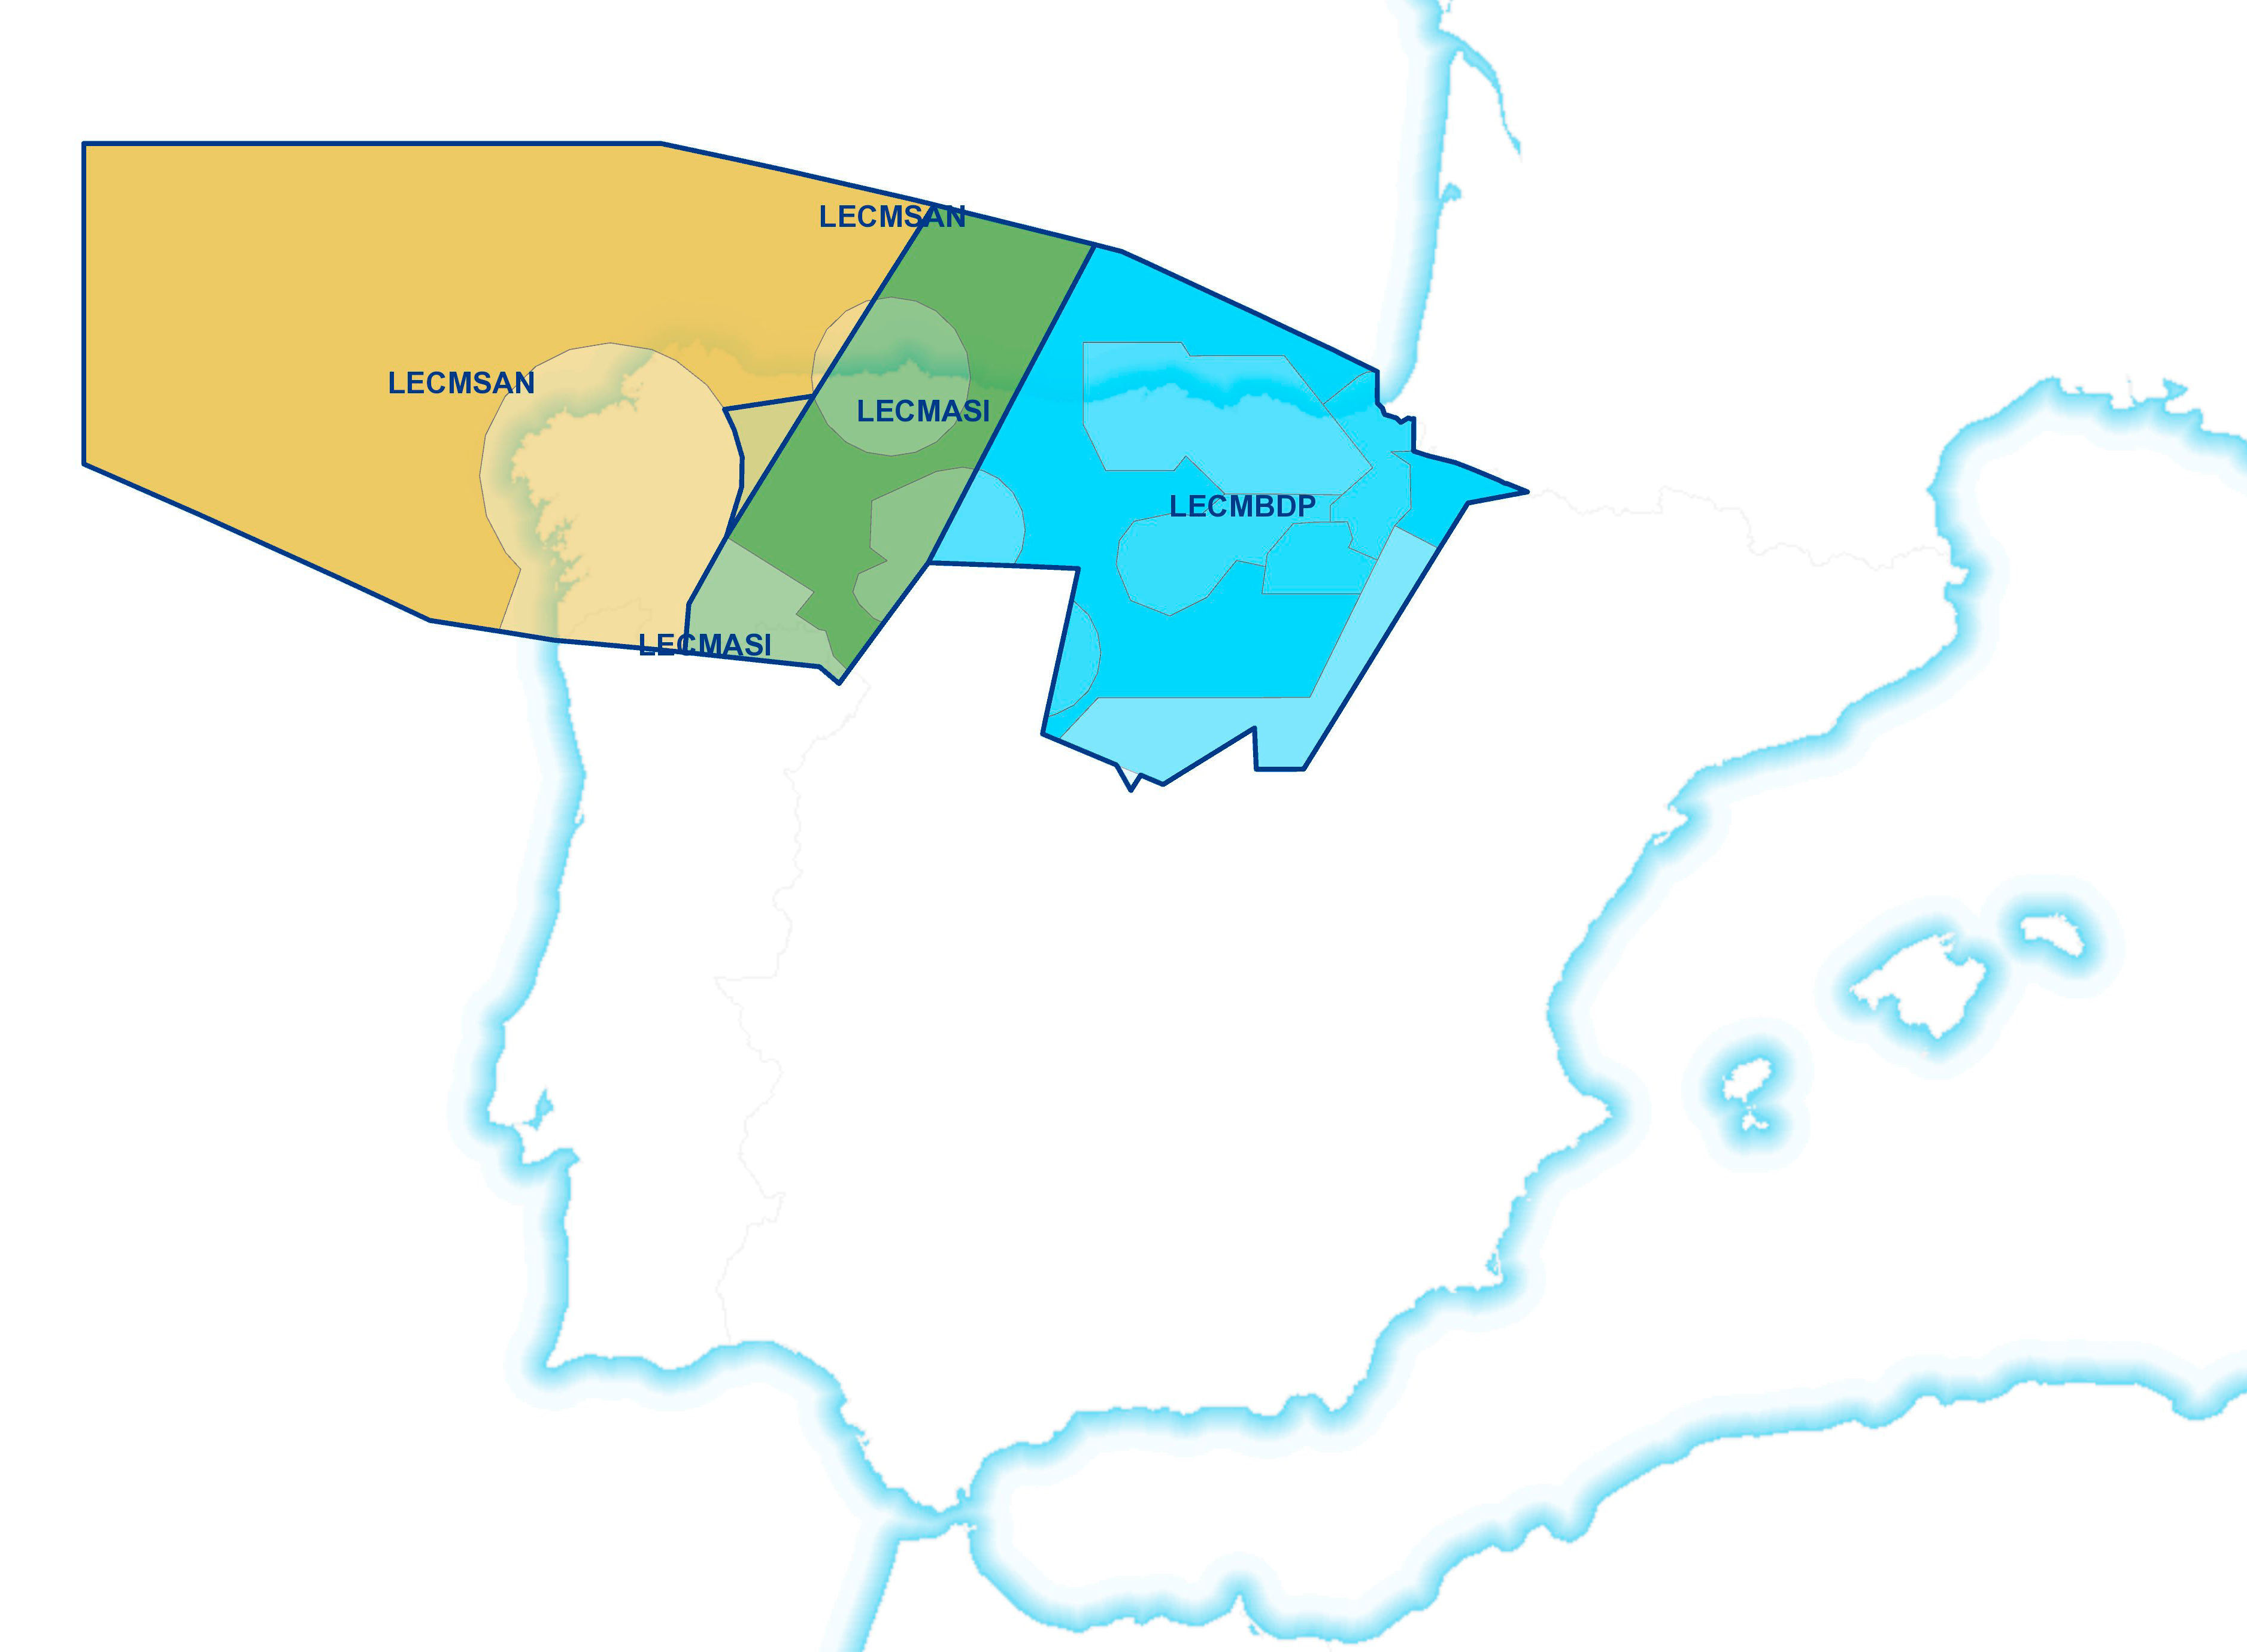
\includegraphics[width=0.6\linewidth]{sectorizacion-3D}
        \caption{sectorizacion 3D\linebreak}
        \label{fig:2:sectorizacion-3d}
    \end{subfigure}

    \begin{subfigure}{\linewidth}
        \centering
        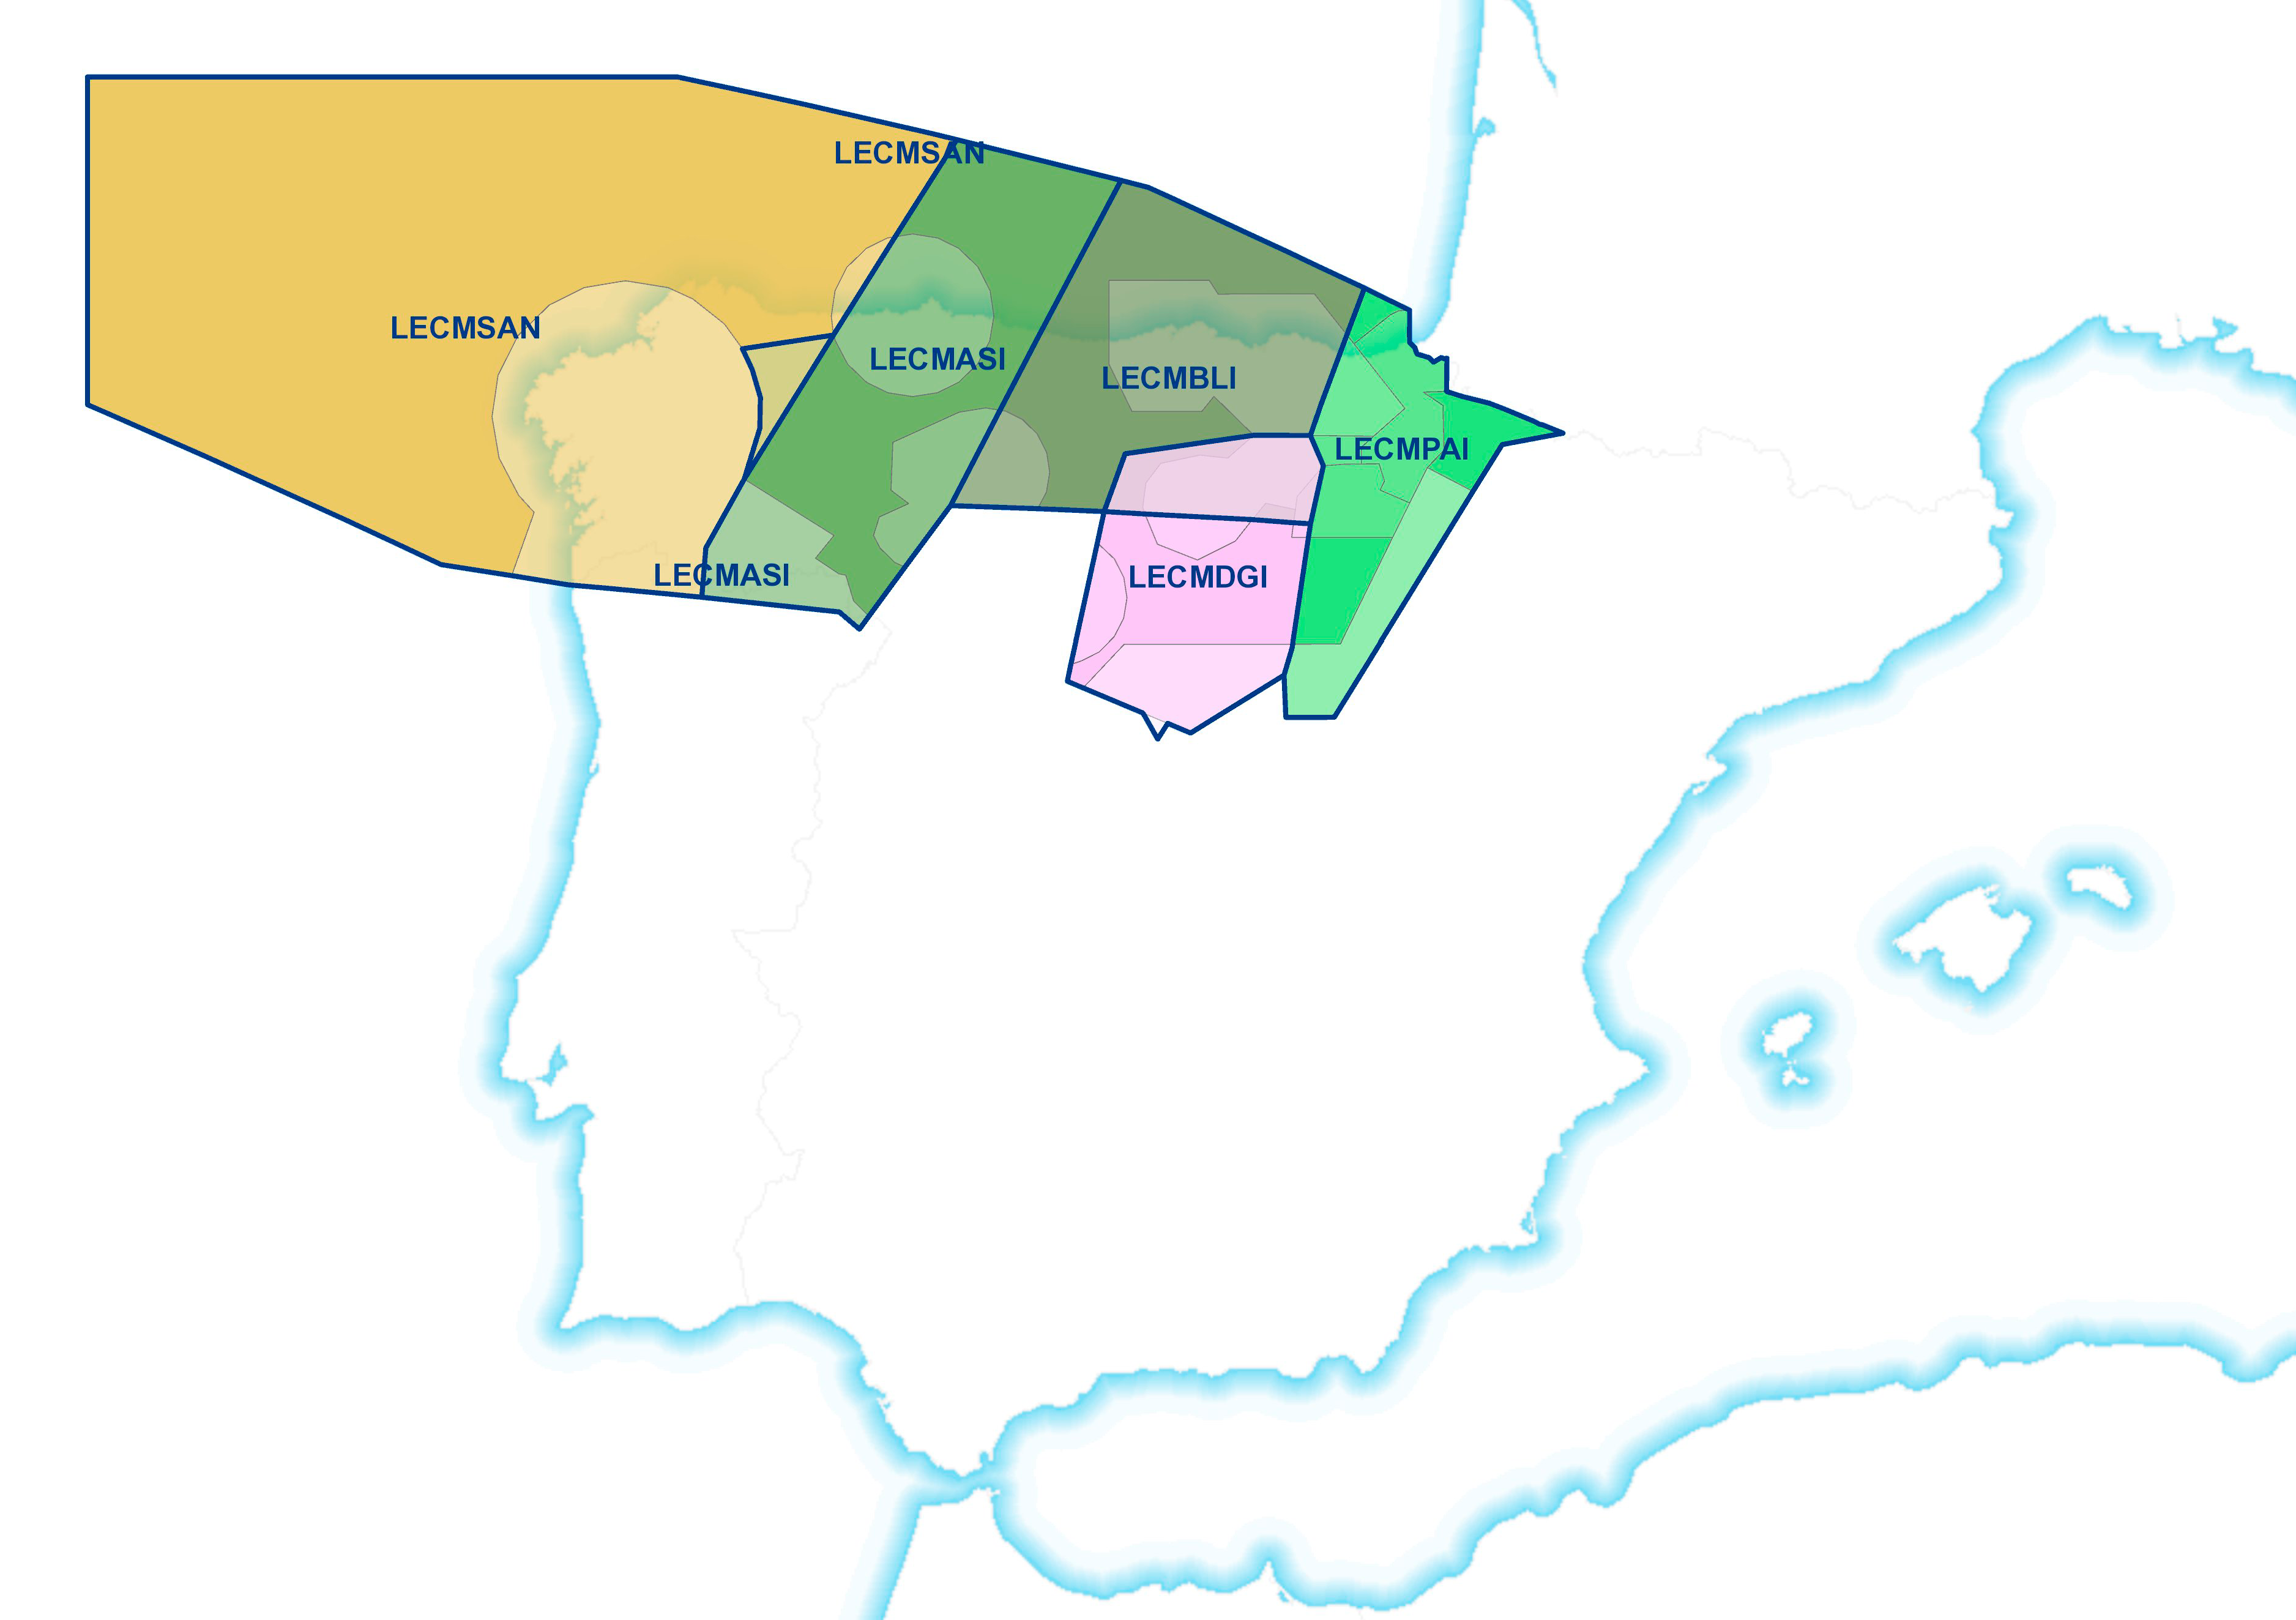
\includegraphics[width=0.6\linewidth]{sectorizacion-5A}
        \caption{sectorizacion 5A}
        \label{fig:2:sectorizacion-5a}
    \end{subfigure}

    \caption{Ejemplo de comparativa de una sectorización 3B y 3D de la dependencia MADRID Ruta 1}
    \label{fig:2:comparativa3B-3D}
\end{figure}


Cuando cambiamos de una configuración de partida a otra, nos encontramos 2 posibles situaciones: que pasemos de una sectorización
con un menor número de sectores a otra con mayor (como en el ejemplo anterior) donde se \textit{abrirán} sectores; o por el
contrario que pasemos de una sectorización con un mayor número de sectores a otra menor (por ejemplo, el caso contrario: de una 5A a una 3D)
donde se \textit{cerrarán} sectores, pero como hemos visto, algunos serán comunes y no sufrirán cambio.
\\

El siguiente concepto importante es el de afinidad entre sectores. Sin entrar en demasiado detalle, la unidad mínima de
división del espacio aéreo son los volúmenes, de esta forma los sectores subirán un determinado número de volúmenes.
Pues diremos que dos sectores \textit{son afines entre sí} si comparten al menos un volumen entre sí. Para saber si dos
sectores son afines, utilizaremos la llamada \textit{matriz de afinidad} que, si bien puede ser construida manualmente,
en nuestro caso será tratada como un input del sistema para ahorrar tiempo innecesario de cómputo, pues es constante para
cada dependencia (en el Apartado XXX se muestra un ejemplo). %TODO referencia!!
\\

Por último, resta introducir el concepto de \textit{núcleo}. Un núcleo no es más que una agrupación de alto nivel de
varios sectores, pudiendo un sector pertenecer a varios núcleos (relación N a N). El uso de los núcleos facilita la
gestión de la acreditación los controladores aéreos, pudiendo estos controlar únicamente un determinado núcleo (ver Requisito XXX.) %TODO referencia


\NOTE{Hasta aquí gramática revisada} %TODO eliminar nota

\subsection{Requisitos del sistema}
Una vez definidos los conceptos básicos, procedemos a recopilar las características y restricciones del sistema.

\subsubsection{Requisitos de entrada/salida}

\begin{enumerate}[label={\textbf{RIO\arabic*}}]
    \item  Una entrada al sistema se compondrá de dos partes: la información de la dependencia y la información del caso,
    de esta forma, la información común a varios casos será independiente de cada caso concreto.
    \item La información de la dependencia será un subdirectorio con el nombre de la dependencia, contendrá 4 ficheros:
    \begin{enumerate}[label*={\textbf{.\arabic*}}]
        \item  Lista de todos los sectores pertenecientes la unidad de control y los sectores elementales\footnote{
        Sector que comprende una zona del espacio aéreo que no es subdivisible empleando otros sectores. Recuérdese el sector LECMBDP (azul) de la \autoref{fig:2:sectorizacion-3d} se podía sustituir por otros más pequeños, por lo tanto no es elemental
        } por los que están formados cada uno de los sectores.

        \item  Matriz de Afinidad de los sectores de la dependencia (definida en la \autoref{section:2:sectores-y-sectorizacion})
        \item Lista de los sectores pertenecientes a la unidad de control, en la que nos indica el tipo de sector (ver~\ref{RD-tipos-sector}) y los núcleos a los que pertenece (ver~\ref{RD-sector-nucleo}).
    \end{enumerate}

\end{enumerate}


\subsubsection{Restricciones de dominio}
Las restricciones de dominio son aquellos requisitos del sistema que son impuestos únicamente por el dominio del problema, no por la propia naturaleza del sistema ni de forma externa.

\begin{enumerate}[label={\textbf{RD\arabic*}}]
    \item \label{RD-tipos-sector}  Cada sector tendrá un tipo de sector, que podrá ser Aproximación o Ruta
    \item  \label{RD-sector-nucleo} Cada sector tendrá uno o varios núcleos asociados, asi como cada núcleo tendrá un conjunto de sectores (relación N a N)

\end{enumerate}













